\documentclass[12pt]{article}

\usepackage{fullpage}
\usepackage{epsfig}
\usepackage{graphicx}

\newcommand{\code}[1]{\texttt{#1}}

\author{Marc G. Bellemare, Adam White, Mike Sokolsky}
\title{The RLAI Robotic Simulator\\ A Tutorial}

\begin{document}
\maketitle

\section{Introduction}

This tutorial documents the RLAI Robotic Simulator: how to install it, how
to run it and how to use it in your work. After installing the simulator
you will have a choice of operating it in Normal mode (involving an agent
and a reward function) or in Standalone mode, where you can personally 
control the robot in the environment. After performing the installation
(Section \ref{sec:installation}),  I suggest running the simulator in 
Standalone mode (see Section \ref{subsec:standalone}) once initially to get
an idea of the environment in which the robot lives. 

\section{Requirements}

\begin{itemize}
\item{Java 1.5}
\item{Make and g++}
\item{A POSIX Operating System (Mac OS X, Linux, BSD...)}
\end{itemize}

\section{Installing the Simulator}\label{sec:installation}

Installing the simulator is a matter of a few steps. In order, you should:

\begin{enumerate}
\item{Download the Simulator package}
\item{Build the DisCo framework}
\item{Copy relevant files into the Simulator}
\end{enumerate}

Each step will be detailed in the following sections with instructions for
UNIX systems.

\subsection{Downloading and installing the RLAI Robotic Simulator}

If you have not yet downloaded it, the Simulator package can be found at 

\begin{verbatim}
http://www.cs.ualberta.ca/~mg17/critterbot/files/RLAISimulator.tgz
\end{verbatim}

For the remaining of this tutorial, I will assume that you have downloaded
this file to a directory called \verb+robots+. Assuming that this is done, 
you should extract files from the tarball:

\begin{verbatim}robots> tar -xvzf RLAISimulator.tgz \end{verbatim}

The simulator itself, being in Java, does not need to be compiled. Before
we actually use it, however, we need to set up the framework, called DisCo,
that binds the simulator, the agent and the reward generator together.

\subsection{Building DisCo}

According to its website, DisCo is a ``framework for developing and running 
applications that must process data which is being produced in real time.'' 
For now we will not
concern with the details of what the framework does; you can learn more at
\begin{verbatim}http://www.cs.ualberta.ca/~roberts/intro.html\end{verbatim}.

Thankfully, \verb+RLAISimulator.tgz+ comes with a pre-packaged version of 
DisCo, extended with Critterbot-specific files. The files of interest are in
a subdirectory \verb+disco+. Before compiling the framework, you need to copy 
a file specifying some information about your operating system (DisCo is meant
to be cross-platform). Depending on your operation system, the file in 
question is:

\begin{itemize}
\item{\textbf{Linux}: LIBSLINUX.d}
% UNIX?
\item{\textbf{Mac OS}: LIBSMAC.d}
\item{\textbf{Windows}: Out of luck.}
\end{itemize}

Assuming a Linux machine, execute the following:

\begin{verbatim}
robots> cd disco
robots/disco> cp make/LIBSLINUX.d make/LIBS.d
\end{verbatim}

On a Mac OS-based machine, you would replace LIBSLINUX.d by LIBSMACS.d. We 
are now ready to build:

\begin{verbatim}
robots/disco> make

<crunch crunch crunch>

robots/disco> cd ..
robots>
\end{verbatim}


\subsection{Copying relevant files to the RLAI Robotic Simulator}

There is a single file of interest in the DisCo directory, located in the
\verb+bin+ directory and named \verb+Control.bin+. If you extracted the 
DisCo code to its default directory, \verb+disco+, then the file should 
be located at \verb+disco/bin/Control.bin+.

All that is needed is to copy the file over into the Simulator directory.
Assuming the installation directory for the Simulator is \verb+simulator+,
then you can copy the file as follows:

\begin{verbatim}
robots> cp disco/bin/Control.bin simulator/bin/Control.bin
\end{verbatim}

This completes the installation! 

\section{Running the Simulator}

Provided that you installed all the required files, you should now be able to
run the Simulator out of the box. There are two possible modes of operation,
namely standalone mode and normal mode. In standalone mode only the simulator
itself will be running, without an agent or a source of rewards. In this mode
you can control the robot manually using the arrow keys. On the other hand,
in normal mode the Agent program (\verb+src/Agent.java+) controls the robot.

Playing with the simulator in standalone mode can give you an idea of how the
robot moves around and how objects react before designing an agent.

\subsection{Standalone Mode}\label{subsec:standalone}

The following will start the simulator in standalone mode:

\begin{verbatim}
robots> cd simulator 
robots/simulator> ./runStandalone.sh
\end{verbatim}

The \verb+runStandalone.sh+ script will compile the simulator loader,
\verb+src/Simulator.java+, and execute it. The specifics of this program will 
be detailed later in this tutorial.

Once you execute \verb+runStandalone.sh+, you should see a GUI appear, showing
the state of the simulator. The arrow keys will drive the robot around. Some 
of the
sensory information is currently drawn (such as bump sensors), but we do not
aim to provide a complete visualization of the data. You can also drive the
robot around using the ASDQWE keys, which provide three degrees of freedom
(by adding lateral motion).

\subsection{Normal Mode}

The following will start the simulator in normal mode:

\begin{verbatim}
robots> cd simulator 
robots/simulator> ./run.sh
\end{verbatim}

The \verb+run.sh+ script will compile three Java files, namely

\begin{itemize}
\item{\verb+src/Simulator.java+}
\item{\verb+src/Agent.java+}
\item{\verb+src/RewardGenerator.java+}
\end{itemize}

These files respectively create the simulator, a simple agent and a reward
generator. By default they open up ports 2324, 2325 and 2326. You can modify
these ports (see Section \ref{sec:changingDefaults} for more information).

After compiling the Java sources, the script will run the corresponding
binaries and the DisCo binary \verb+Control.bin+. The latter is in charge
of the communication between the three components. The script will then wait
for any of the four processes to die, at which point it will attempt to 
terminate all of them.

Once you start \verb+run.sh+, you should see a GUI appear (provided you are
running on a machine with a display). Figure \ref{fig:gui} shows a sample
snapshot from the GUI with details about the various components.
The arrow keys are disabled in Normal Mode to prevent competition for control 
between the agent and the user. 
By default the Agent will send commands at regular intervals;
you should see the robot performing some behavior which depends on the mood
of the programmer at the time the simulator was packaged. Section 
\ref{sec:writingAgentAndRewardGenerator} discusses the provided agent and
reward generator as well as how you may modify them. 

\begin{figure}\label{fig:gui}
\centerline{
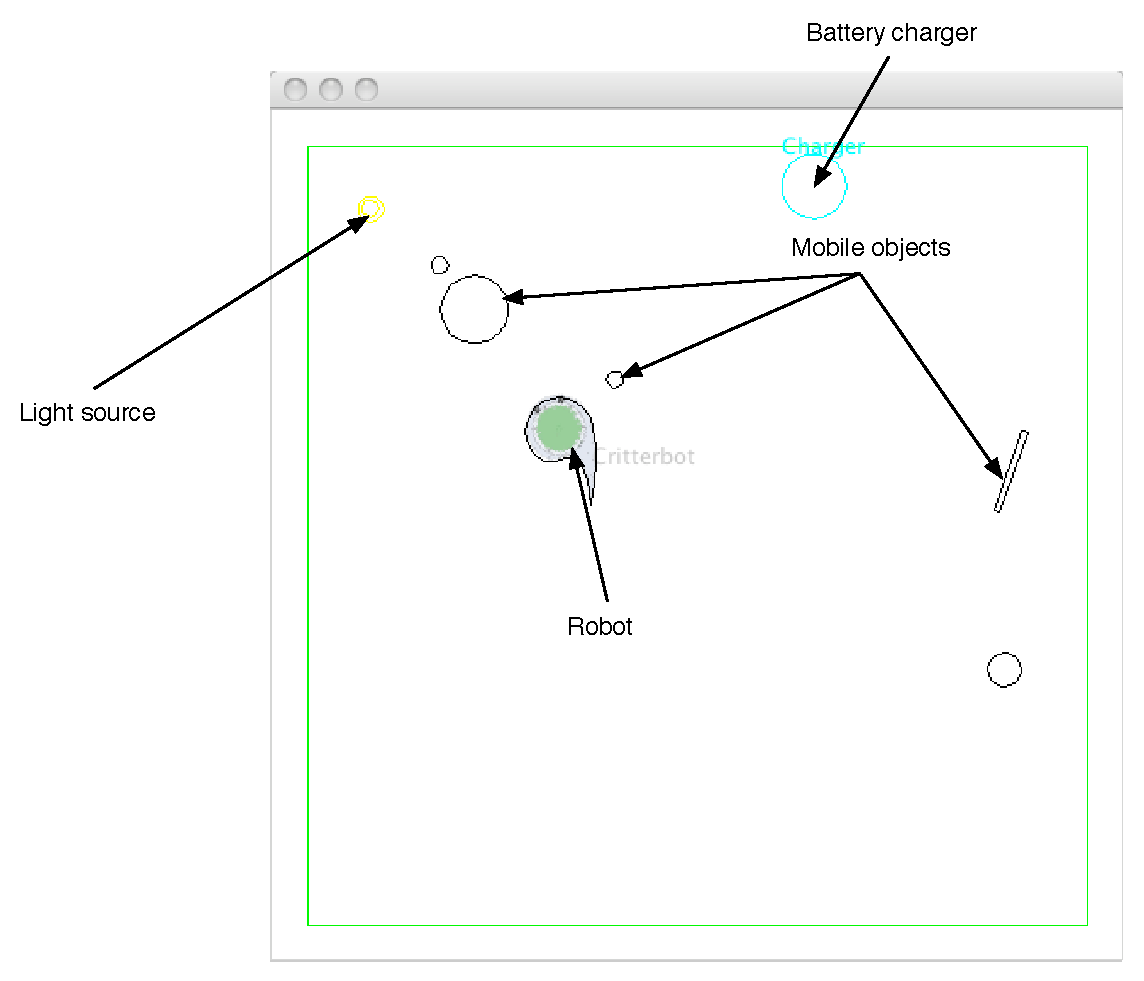
\psfig{file=images/Simulator_GUI.pdf,width=5in}
}
\caption{The RLAI Robotic Simulator Graphical User Interface.}
\end{figure}

\section{Agents, Environments and Reward Generator}\label{sec:writingAgentAndRewardGenerator}

\subsection{Introduction}\label{subsec:programming_introduction}

Within the simulator package each of the basic signals in reinforcement learning (actions, observations, rewards) is a separate class.  Individual instances of data are known as Drops, terminology borrowed from Disco, so we are interested in \verb+CritterControlDrop+s, \verb+CritterStateDrop+s, and \verb+CritterRewardDrop+s.  It is well worth a few minutes to read over the documentation on the content of these drops at:

\begin{verbatim}
http://www.cs.ualberta.ca/~sokolsky/critterbot/interface.php
\end{verbatim}

Disco takes care of distributing the data to classes that are interested in it, so all you have to worry about is choosing the reward value and generating actions to be implemented on the robot.  Read the following section even if you plan on developing in C++ as it contains some useful information about how the system is organized.

\subsection{Java}\label{subsec:java_agent}

If you are using Java, the two files you are interested in will be in the \verb+src+ directory.  Lets first take a look at \verb+RewardGenerator.java+.  Most of this file is machinery for moving the data around, we are mostly interested in the \verb+parseStateDrop+ method.  It takes in a CritterStateDrop and should set the value of \verb+aReward+ before returning.  You have access to all the information in the CritterStateDrop, documented at:

\begin{verbatim}
http://www.cs.ualberta.ca/~mg17/critterbot/docs/
\end{verbatim}

There are two very simple examples already in the file, one generates a reward proportional to the front facing light sensor, the other a binary reward if a bump sensor is activated or not.  Keep in mind that in the simulator environment the bump sensor values are 0 when inactive, while in a real-world environment they would likely always have some low noisy value.  You are welcome to create significantly more complex generators for reward signals, depending on the task.

The file we are most interested in is \verb+Agent.java+, where your learning agent lives.  There are a few places here you'll be adding code, and will likely add more methods and external classes when creating an agent of any complexity.  The first place to look is at the \verb+parseStateDrop+ method.  Data is provided here in Drop form, and generally for reinforcement learning we'd like it as a simple vector.  The double vector \verb+aObservation+ is available to save whatever fields from the drop you would like to use as part of your state observation.  If you prefer, feel free to save the drop itself in an instance variable and use it instead of the \verb+aObservation+ vector.

Finally we get to the actual learning code.  There is a method named \verb+act+, a term also inherited from Disco.  This method gets called repeatedly, so we wait until we've collected a new observation and reward before proceeding.  Now you get to run code you want called each timestep.  In the example we create a very simple behavior, the robot can either drive forward or backward, and changes direction every time it received a non-zero reward.  Once we return from this method the \verb+CritterControlDrop+ that was just created gets passed on to the robot itself.

Executing the \verb+run.sh+ script will automatically recompile these two files and start the simulator and your agents running.

\subsection{C++}\label{subsec:cpp_agent}

Programming in C++ means interacting directly with Disco.  Like in Java the reward generator is separate from the agent, but we now have four files, two cpp files and two header files, located in \verb+disco/source/critterbot+.  In RewardGenerator.cpp there are two methods you will probably modify.  \verb+init+ is as expected, do any variable or other initialized here.  The \verb+update+ method is called when there is a new observation to create a reward from, and that observation is available to you in the instance of \verb+stateDrop+.  This follows the same structure as the Java state drop, for details see \verb+CritterStateDrop.h+ in the same directory.

Your agent will live in \verb+CritterAgent.cpp+, and as in \verb+RewardGenerator.cpp+ any initialization should be put in \verb+init+, which will be called once at startup.  The agent itself will run out of the \verb+update+ method, here you have access to both the state observation information and the reward, and should write whatever values you want to the \verb+controlDrop+ instance.  Details on the C++ control drop are, amazingly enough, found in \verb+CritterControlDrop.h+ in the same directory.

The script \verb+runDisco.sh+ will try to compile your C++ agent and reward code and run it in the simulator.  -IMPORTANT NOTE-  The makefile used by Disco only looks for changes to .cpp files.  If you only edit a header file it will not automatically recompile your code, so be sure to touch the related .cpp file.

\subsection{Errata}\label{subsec:programming_exercises}

You may have noticed watching the default agent that it doesn't always change direction immediately after running into something.  This is because the bump sensor values decay a little after impact before returning to zero, meaning the agent receives several sequential non-zero rewards.  Depending on if there are an even or odd number of these the agent may or may not start moving in the opposite direction.

Both the robot and the simulator are real-time systems, so interacting with them is necessarily asynchronous.  Nothing is going to wait for you to finish some time-intensive computation, so it is highly recommended not to allow your code to block.  If one or more observations occur while your agent is still processing data they will be discarded, only the most recent observation is provided when your agent is called.  Depending on what your agent does this may or may not be a problem.  Spawning a separate Java thread is one possible way to do long-term processing, it is beyond the scope of this document to describe but Disco also allows externalizing complex processing to a separate process.

Another result of the asynchronous environment is that you cannot rely on an ordering of events.  Don't expect your agent code to be called exactly on the 10ms mark, between the OS scheduler and TCP transport delays there will likely be some variation.  The code is currently written so your agent always receives a new observation and reward drop together, but be aware the reward may be slightly out of phase with the observations; the reward may actually be generated by an observation one or two time steps in the past.  Remember, you don't have to use a separate reward generator, you can do the reward calculation direction in your agent, it is simply there as a useful abstraction.

\subsection{Environments}

Writing environments is not as straightforward in the provided package as it
is to write an agent or a reward generator. However, we are providing a few
default environments (Table \ref{table:environment_list}) with which users may 
play. Replacing the environment that is loaded simply involves changing 
which environment is created in the main method() of \verb+Simulator.java+.
In particular, in the line

\begin{verbatim}
final SimulatorEngine engine = 
  createSimulatorEngine(dropInterface, new SimpleEnvironment());
\end{verbatim}

\verb+SimpleEnvironment+ may be replaced by another environment class name
from the given list.

\begin{table}
\small{
\begin{tabular}{|c|c|}
\hline
\code{SimpleEnvironment} & The default environment - \\
& some objects, a light source and a battery charger \\
\hline
\code{FunEnvironment} & Same as SimpleEnvironment, but with more objects \\
\hline
\code{RobotOnlyEnvironment} & An environment with a robot and nothing else \\
\hline
\code{BasketBallEnvironment} & A robot, a ball and some form of basket \\
\hline
\code{LightBatteryEnvironment} & An environment with a battery charger and five light sources \\ 
\hline
\end{tabular}
}
\caption{A list of available environments for the simulator.\label{table:environment_list}}
\end{table}

\section{Default Parameters and Command-Line Arguments\label{sec:changingDefaults}}

\subsection{Simulator}\label{subsec:simulator_parameters}

The following command-line arguments can be used with \verb+Simulator.java+:

\begin{center}
\begin{tabular}{|c|l|}
\hline
\verb+-p [port]+ & specifies which port the Simulator should listen on. Default: 2324. \\
\hline
\verb+-ng+ & disables the GUI (and keyboard control). \\
\hline
\verb+-nk+ & disables controlling the robot via the keyboard. \\
\hline
\verb+-s [scale]+ & specifies the time scale (see below for details). Default: 1.0. \\
\hline
\verb+-h+ & provides help on command-line options \\ 
\hline
\end{tabular}
\end{center}

The time scale $s$ is specified in relative speed of the simulator with respect 
to wall clock. If $s=1.0$, 1 second of simulator time is simulated in 1 second
of wall time. If $s=0.5$, 0.5 second of simulator time is simulated in 1
second of wall time. Values larger than $1.0$ may tax the processor too much,
in which case the simulator will report `Running behind' and slow down.

\subsection{Agent}

In order to modify the port on which the Agent listens, the file 
\verb+Agent.java+ will have to be modified and the variable \verb+discoAgentPort+ changed to a different value.

\subsection{Reward Generator}

In order to modify the port on which the Reward Generator listens, the file 
\verb+RewardGenerator.java+ will have to be modified and the variable 
\verb+discoRewardGeneratorPort+ changed to a different value.


\subsection{DisCo}

The configuration for DisCo may be found in 
\verb+robots/simulator/bin/simulator.xml+. It is beyond the scope of this
tutorial to detail how DisCo should be configured. Of chief interest are the
ports that DisCo connects to. By default these will be 2324, 2325 and 2326.
If modifying the ports for either the Simulator, Agent or Reward Generator,
the DisCo configuration file will also have to be modified accordingly.

\section{Logging and Common Error Messages}

The output of all processes (there are four of them) is redirected by default
to files in the directory \verb+simulator/logs+. In this section we review
what kind of messages you should expect to see if you take a peek at one of
the output logs.

\subsection{Simulator}

The log file for the simulator is \verb+simulator/logs/Simulator+. The 
simulator, like all pieces of software, is not perfect. The most common
error message you are likely to see is

\begin{verbatim}
Simulator is running behind...(actual time scale: 3.55)
\end{verbatim}

This is the simulator's way of telling you that it is unable to simulate
at the requested speed. The easiest way to get rid of it is to reduce the
time scale at which the simulator is asked to operate (below 1.0 if necessary).
The actual time scale reported is the average speed at which the simulator
has operated since it was started. In any event, no harm is caused; the 
simulator will trudge along as fast as it can.

\subsection{DisCo}

The log file for DisCo is \verb+simulator/logs/Disco+. DisCo actually generates 
a lot of output, including information about the data
that is being passed around. A discussion on the Drop data structure and how 
it is handled by DisCo is beyond the scope of this tutorial. However, most of 
the data in the DisCo log file should be easily interpreted.

\section{Final Notes}

The provided package is meant to be easy to install and use. Most likely,
however, you will want to run the Agent (and maybe the RewardGenerator) in
a separate console in order to more easily debug it.

If you have any concerns or questions about the package or the simulator,
you should contact Marc G. Bellemare (\texttt{mgbellemare \_at\_ ualberta.ca}) or Adam White (\texttt{awhite \_at\_ cs.ualberta.ca}).

The simulator source code is available at

\begin{verbatim}
http://code.google.com/p/rlai-critterbot/
\end{verbatim}

Contributions and suggestions are welcome.

\subsection{Bugs, Caveats and Features}

The simulator, from a RL perspective, is not a Markovian process with respect 
to the provided observation data. This is especially visible when the agent
is required to act at a high frequency (100Hz). In particular, it takes one
time step for an action to be processed - in other words, an action sent at
time $t$ will affect the state transition from $t+1$ to $t+2$. There are many
other quirks waiting to be found.

A known issue with the simulator is that objects will sometimes ``stick'' to the
robot. This will happen when the robot pushes objects with the tip of its tail
while rotating.

\newpage

\section{Files included in this package}

\footnotesize{
\begin{verbatim}
simulator/bin/simulator.xml         - DisCo configuration for the Java agent and reward generator
simulator/bin/discoAgent.xml        - DisCo configuration for the C++ agent and reward generator
simulator/bin/extra.xml             - extra DisCo configuration file 
simulator/libs/sim.jar              - the simulator code
simulator/logs                      - log files directory
simulator/compile.sh                - compiles the Java agent and reward generator
simulator/compileDisco.sh           - compiles the C++ agent and reward generator
simulator/run.sh                    - runs the simulator, the Java agent and reward generator
simulator/runDisco.sh               - runs the simulator, the C++ agent and reward generator
simulator/runStandalone.sh          - runs the simulator in standalone mode
simulator/scripts/includes.sh       - additional variables for the run scripts
simulator/src/Agent.java            - the Java agent code
simulator/src/RewardGenerator.java  - the Java reward generator code
simulator/src/Simulator.java        - the simulator loader

disco                               - the DisCo code
disco/source/critterbot/CritterAgent.{h,cpp} - C++ agent code
disco/source/critterbot/RewardGenerator.{h,cpp} - C++ reward generator code
\end{verbatim}
}

\end{document}
